\chapter{Конструкторский раздел}

В данном разделе будут рассмотрены алгоритмы работы анализаторов.

\section{Общий алгоритм работы программы}

Работу данного предложения можно разделить на следующие шаги.
\begin{enumerate}
	\item Лексический, синтаксический, семантический анализы запроса, полученного на входе.
	\item Генерация запросов к различным СУБД.
	\item Выборка необходимых данных из различных СУБД.
	\item Формирование результата с условием запроса пользователя.
\end{enumerate}

На рисунке \ref{img:img1} представлена схема общего алгоритма работы приложения.

На рисунках \ref{img:idef0_1}-\ref{img:idef0_2} представлена диаграмма в нотации IDEF0 \cite{idef0}.

\begin{figure}[h!]
	\begin{center}
		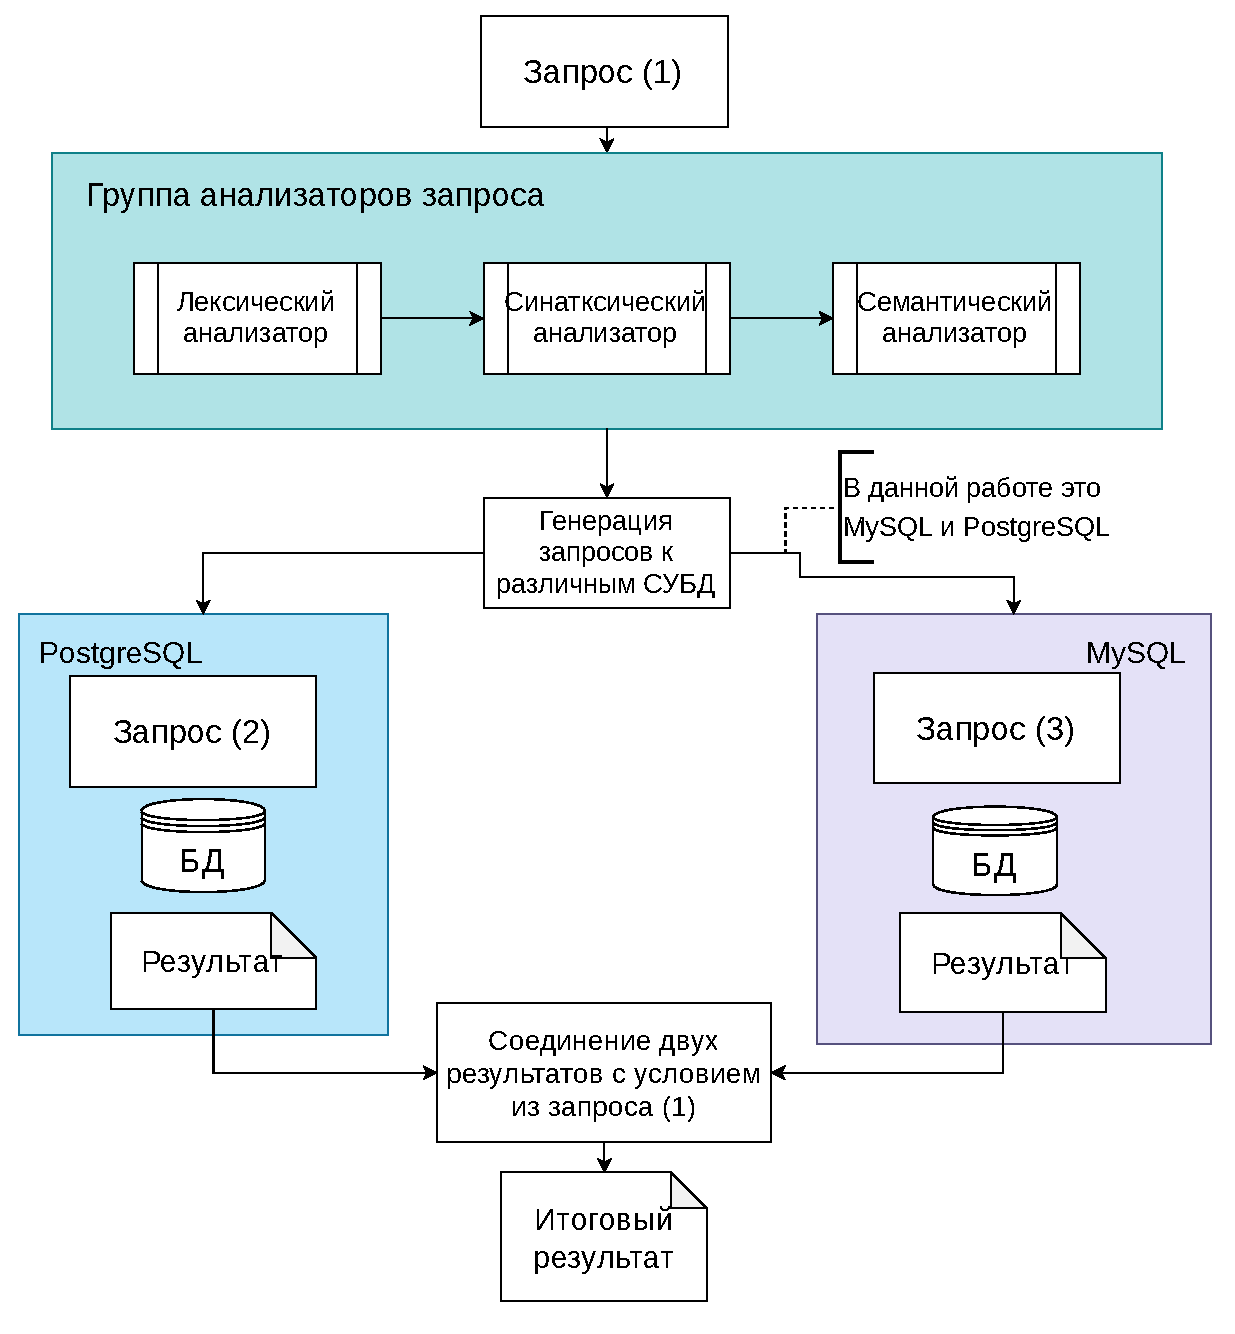
\includegraphics[scale=0.7]{./inc/img/obshalg.pdf}
		\caption{Общий алгоритм работы программы}
		\label{img:img1}
	\end{center}
\end{figure}

\begin{figure}[h!]
	\begin{center}
		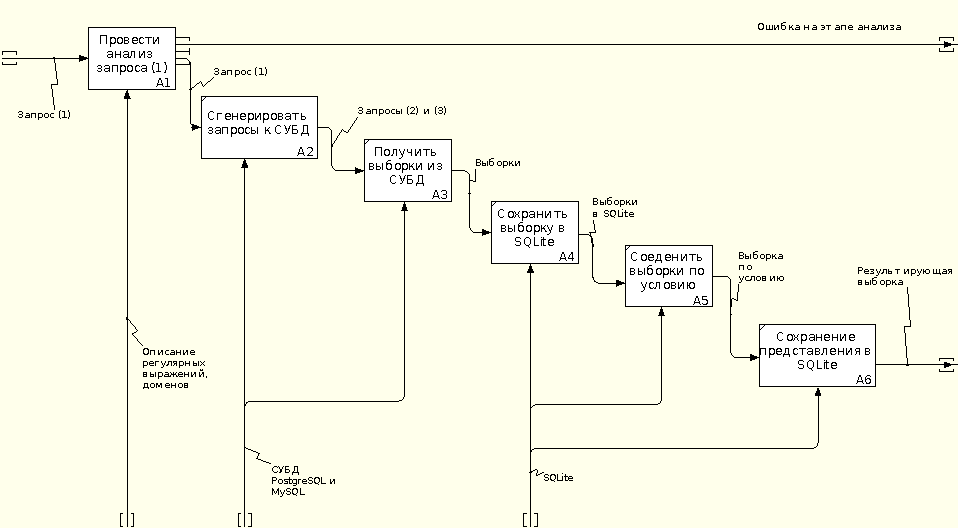
\includegraphics[scale=0.68]{./inc/img/idef0_1}
		\caption{Диаграмма в нотации IDEF0 (1)}
		\label{img:idef0_1}
	\end{center}
\end{figure}

\begin{figure}[h!]
	\begin{center}
		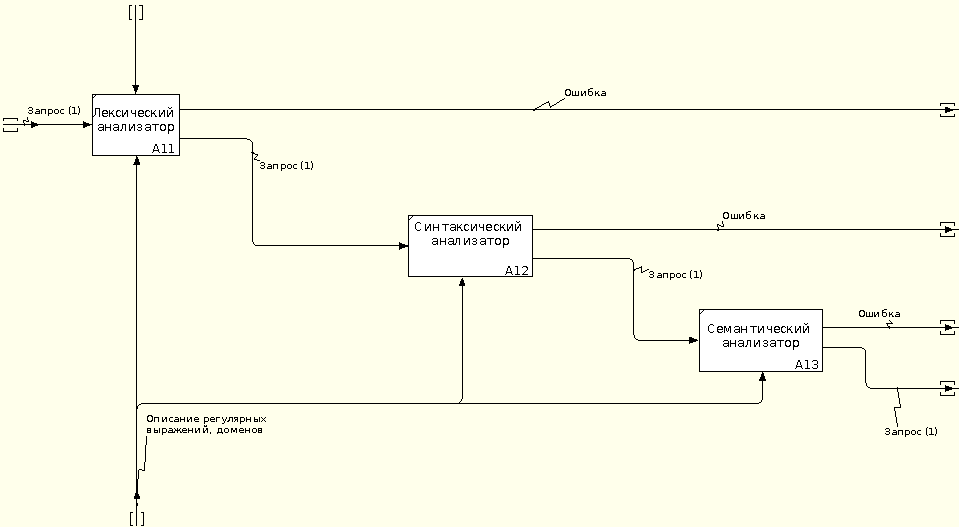
\includegraphics[scale=0.68]{./inc/img/idef0_2}
		\caption{Диаграмма в нотации IDEF0 (2)}
		\label{img:idef0_2}
	\end{center}
\end{figure}


\section{Реализация лексического анализатора}

Основные лексические домены грамматики SQL можно описать при помощи регулярных выражений. На листинге \ref{lst:lex} представлены регулярные выражения для доменов идентификаторов, ключевых слов, целых чисел и чисел и плавающей точкой.

\begin{lstlisting}[label=lst:lex,caption=Регулярные выражения для доменов идентификаторов]
<IDENTIFIER> ::= r'[a-zA-Z_][a-zA-Z_0-9]*|`[a-zA-Z_][a-zA-Z_0-9]*`'

<KEYWORD> ::= r'[a-zA-Z_][a-zA-Z_0-9]*'

<INTEGER> ::= r'(?:[1-9]\d*|0)(?![0-9A-Za-z_])'

<FLOAT> ::= r'(?:([1-9]\d*|0)?\.\d+|([1-9]\d*|0)\.)(?![0-9A-Za-z_])'
\end{lstlisting}


Следует отметить, что лексема числа должна быть разделена от лексемы идентификатора пробельным символом, то есть можно сказать, что не допустима следующая подстрока: <<1234qwerty>>, именно по этой причине в регулярных выражениях есть проверка на символ, следующий за числом.


Чтобы проверить домен на принадлежность к ключевым словам, найденное слово приводится к верхнему регистру и проверяется на принадлежность ключевых слов.

Чтобы сократить затраты ресурсов памяти для компьютера, работа лексического анализатора совмещена с работой синтаксического анализатора. 


В каждый момент работы программы в памяти хранится информация только об одной лексеме, это позволяет сократить затраты памяти. 

На рисунке \ref{img:schema1} представлена схема работы лексического анализатора.

\begin{figure}[h!]
	\begin{center}
		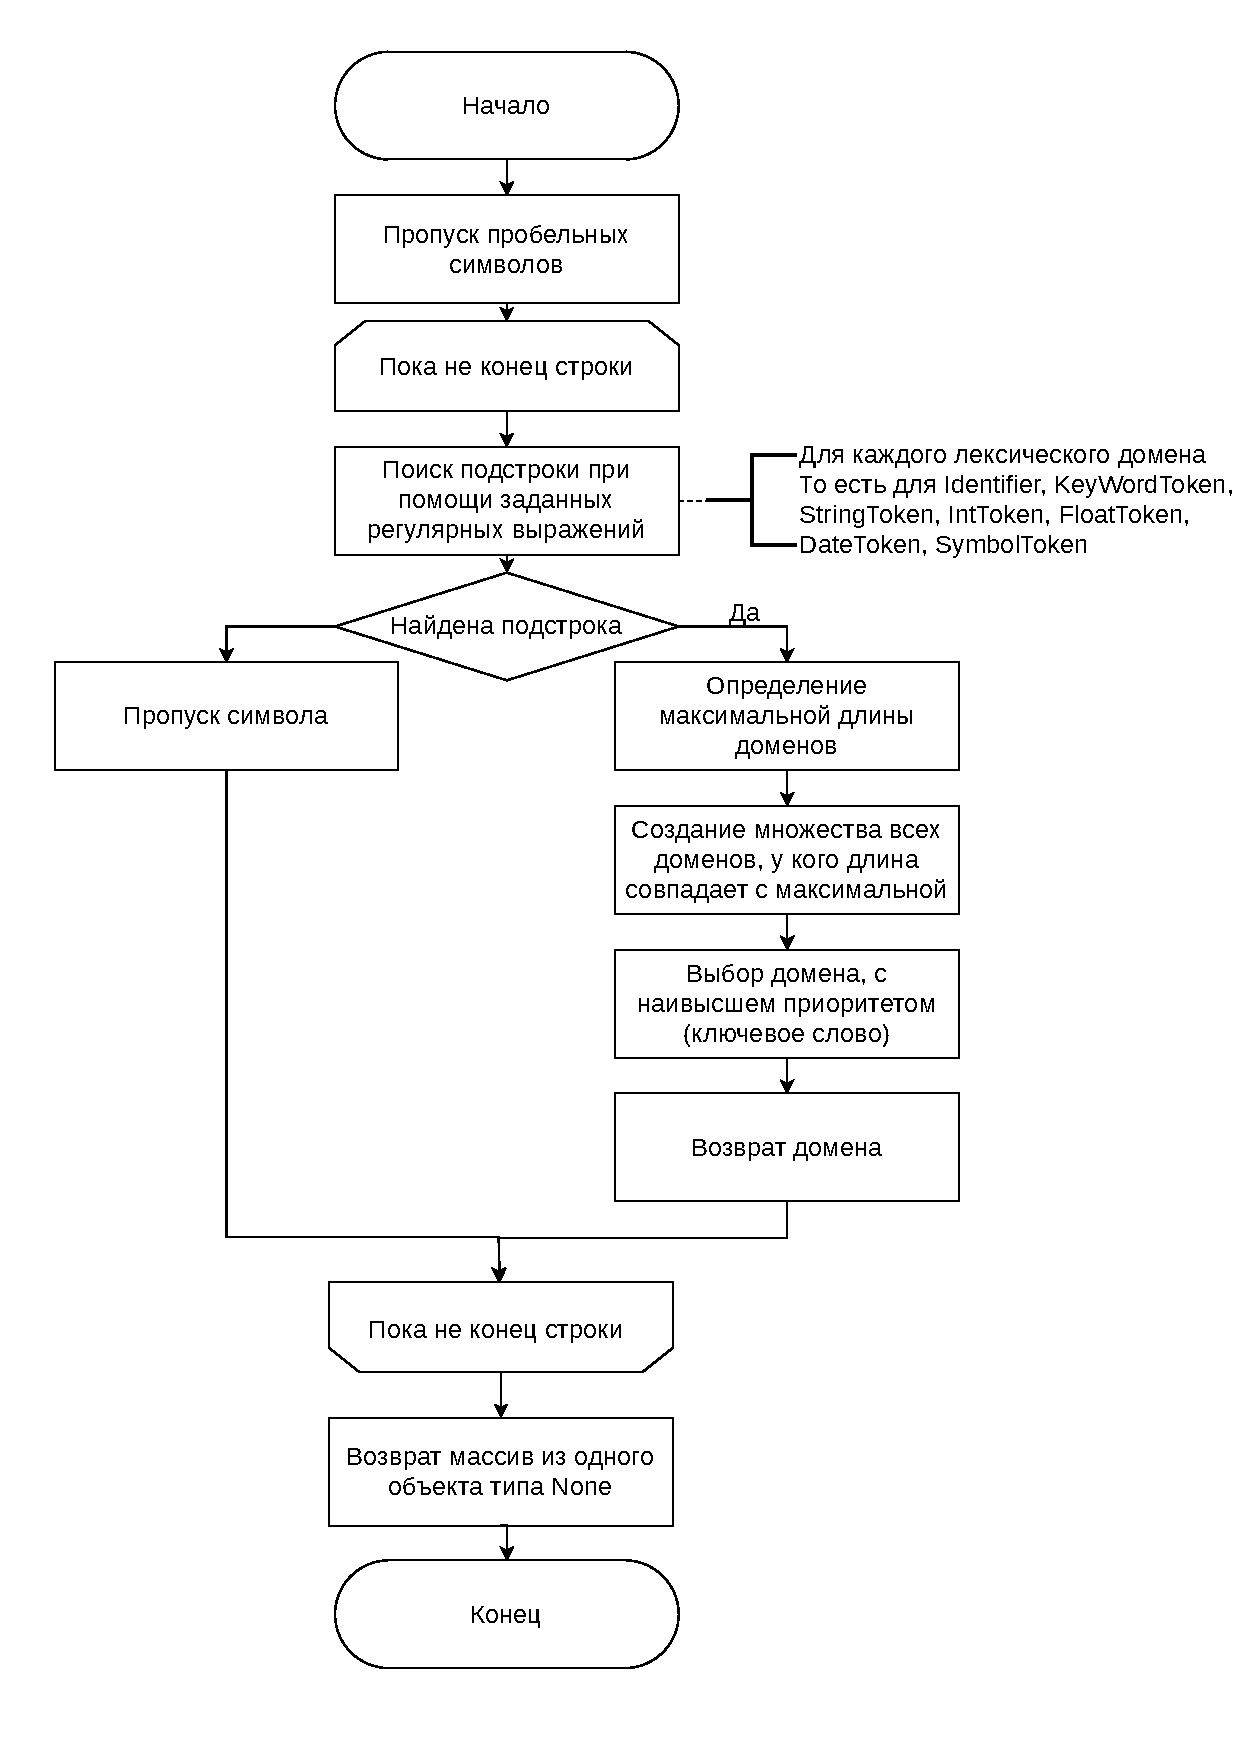
\includegraphics[scale=0.55]{./inc/img/schema1.pdf}
		\caption{Схема алгоритма работы лексического анализатора}
		\label{img:schema1}
	\end{center}
\end{figure}
\newpage


\section{Реализация синтаксического анализатора}

Синтаксический анализатор реализован при использовании метода рекурсивного спуска с возможностью отката. Данный метод просто реализовывать, а также легко расширять путем добавления новых инструкций.


На рисунке \ref{img:schema2} представлена схема работы синтаксической анализатора.

\begin{figure}[h!]
	\begin{center}
		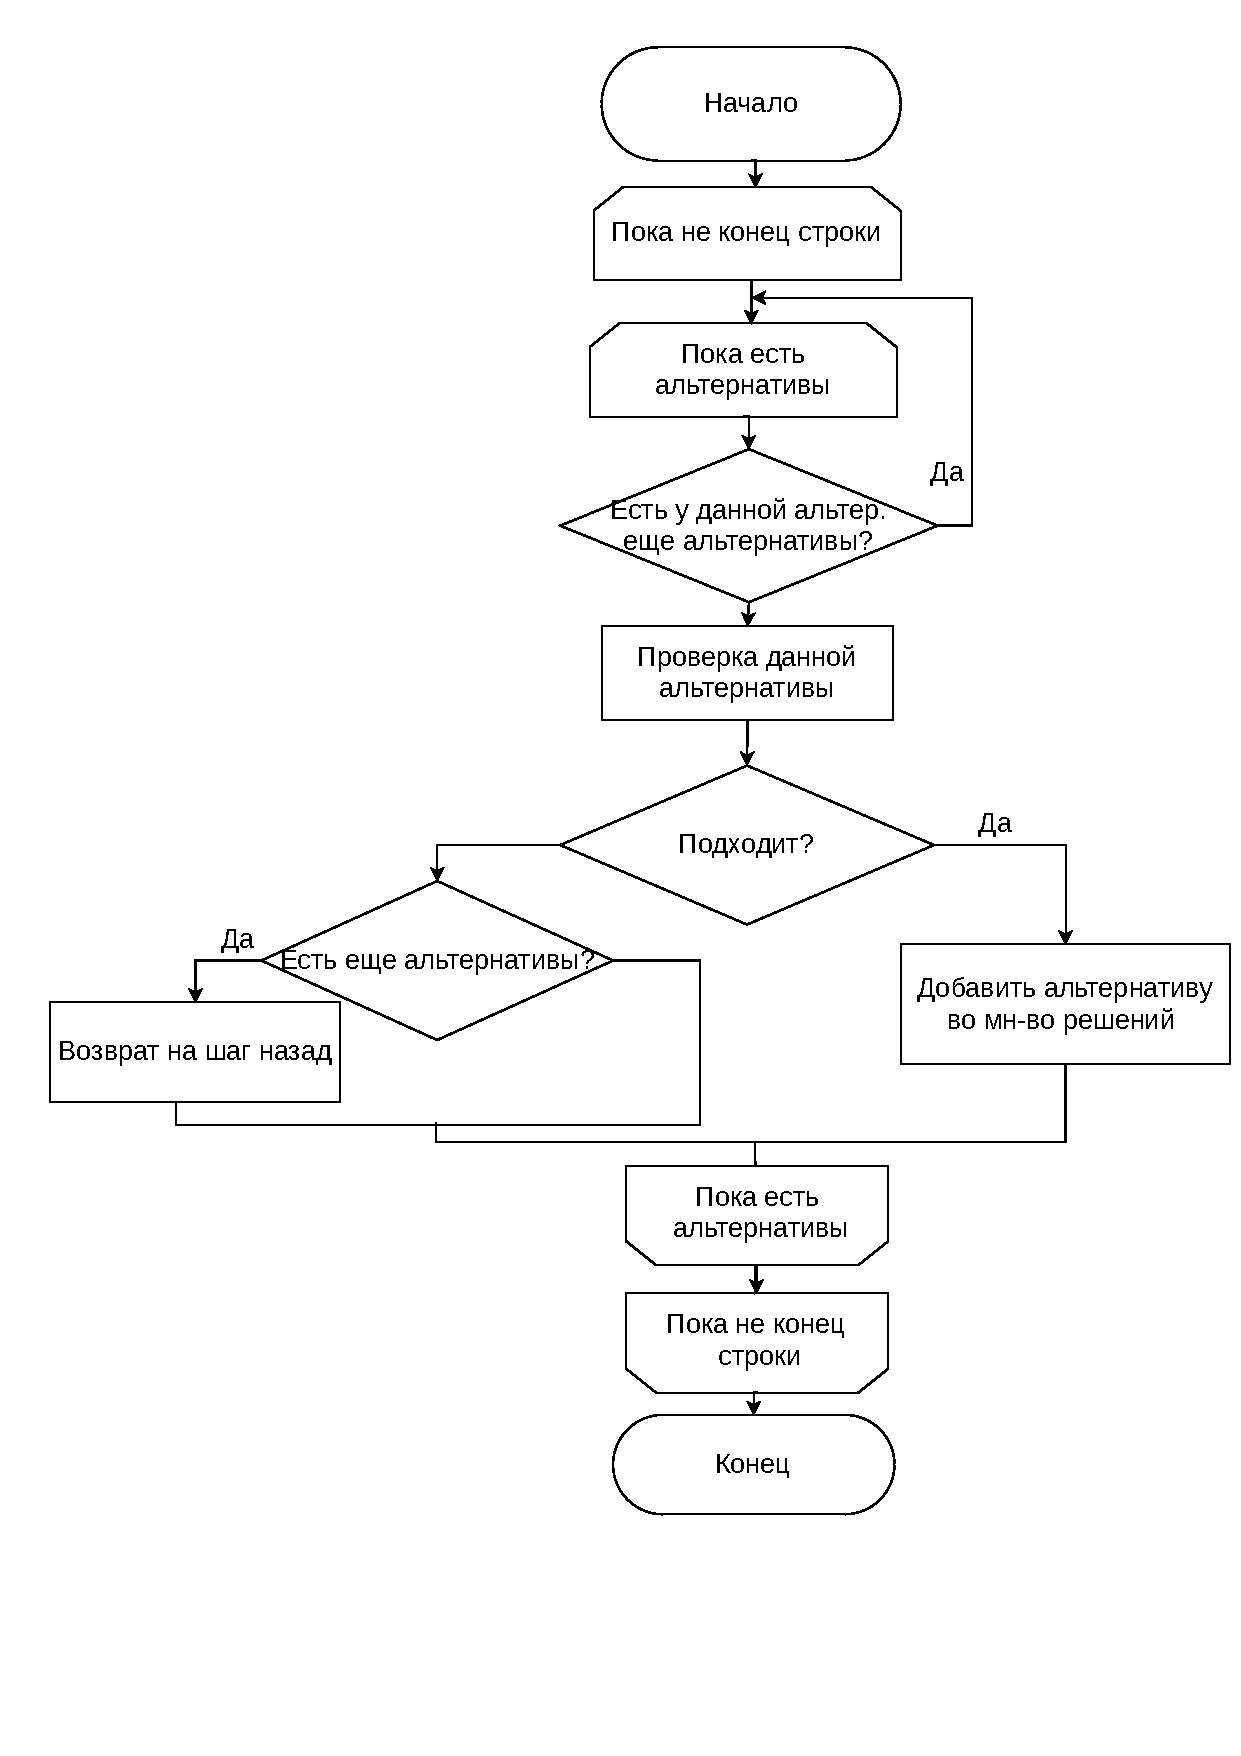
\includegraphics[scale=0.57]{./inc/img/schema2.pdf}
		\caption{Схема алгоритма работы синтаксического анализатора}
		\label{img:schema2}
	\end{center}
\end{figure}

\newpage

\section{Реализация семантического анализатора}

Как было сказано ранее, работа семантического анализа начинается только в том случае, если не было ошибок в работе лексического и синтаксического анализатора.

На рисунке \ref{img:schema3} представлена схема работы семантического анализатора с комментариями.

\begin{figure}[h!]
	\begin{center}
		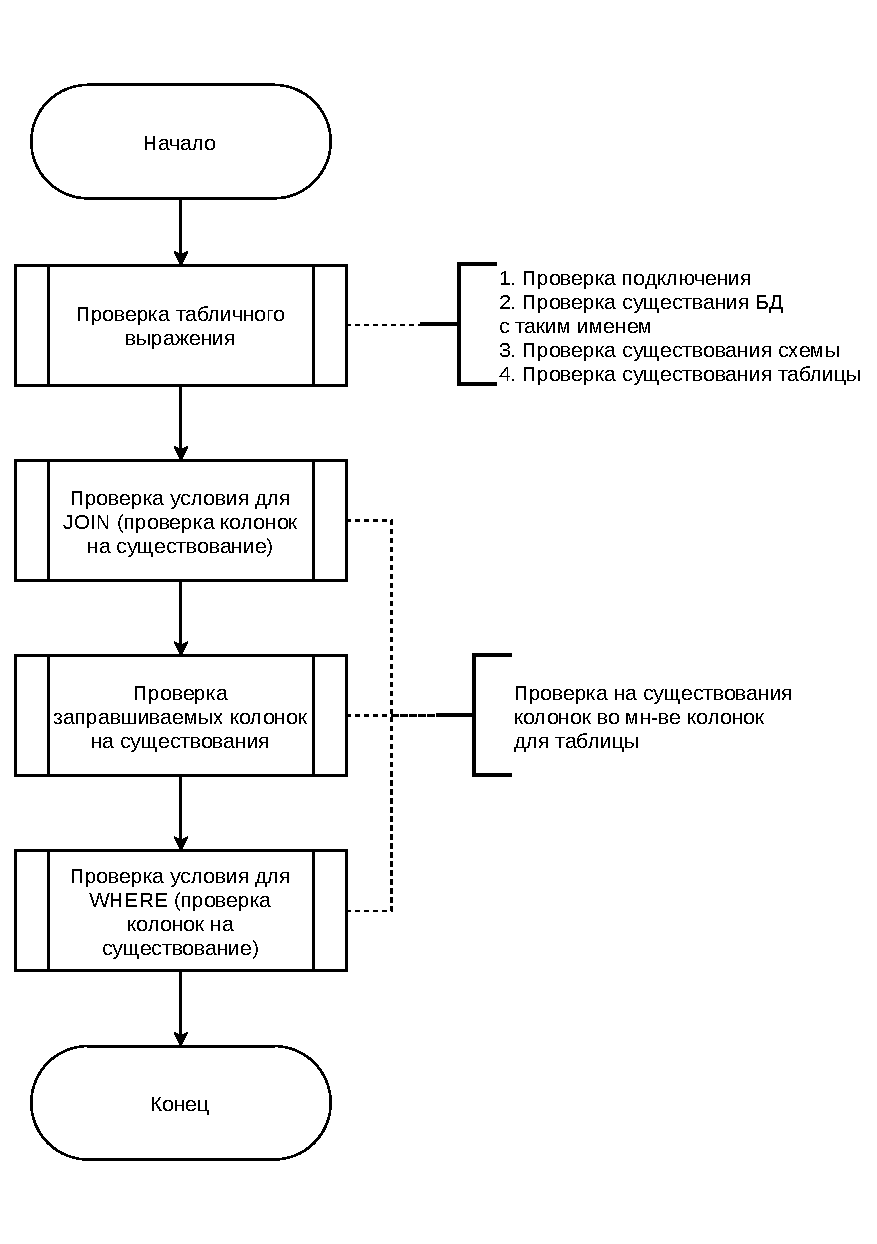
\includegraphics[scale=0.73]{./inc/img/schema3.pdf}
		\caption{Схема алгоритма работы семантического анализатора}
		\label{img:schema3}
	\end{center}
\end{figure}

\section{Формирование и хранение результата}

После получения результатов из PostgreSQL и MySQL, как показано на рисунке \ref{img:img1}, данные переносятся во временную базу данных SQLite \cite{sqlite-standard}.

По умолчанию база данных создается в оперативной памяти, так как это позволяет сократить время, которое тратится на запись в файл и чтение из файла.

Для формирования результирующей выборки в базе данных SQLite определялось представление (VIEW\footnote{VIEW – это хранимый запрос в базе данных.}). Использование представлений позволяет не сохранять результирующую выборку в оперативной памяти, так как ее объем может быть в разы больше чем данные, которые используются при ее построении.

На рисунке \ref{img:idef0_3_res} представлена диаграмма в нотации IDEF0, описывающая процесс формирования и хранения результата в SQLite.

\begin{figure}[h!]
	\begin{center}
		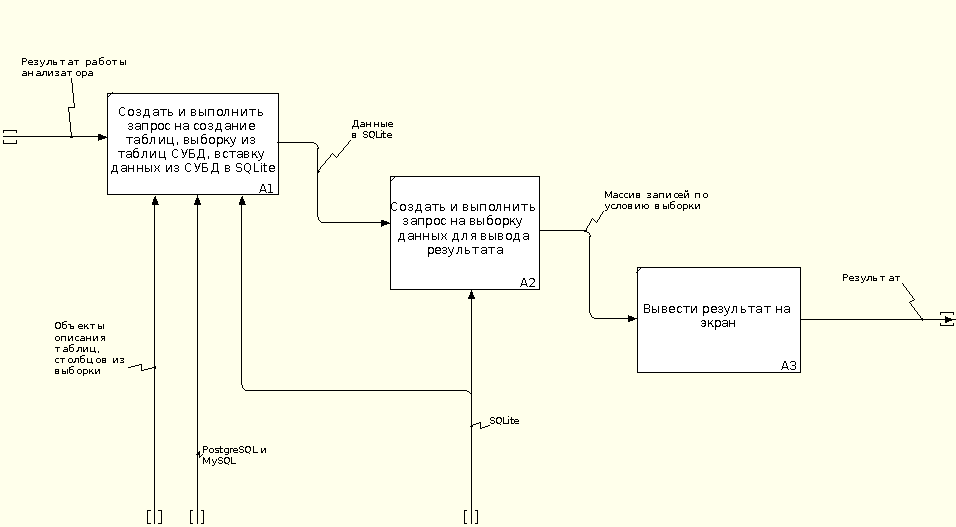
\includegraphics[scale=0.68]{./inc/img/idef0_3_res}
		\caption{Описание процесса формирования и хранения результата в SQLite}
		\label{img:idef0_3_res}
	\end{center}
\end{figure}

В данной работе предусматривается, что данных, хранящихся в MySQL и PostgreSQL, гарантированно меньше, чем объем оперативной памяти.


\section{Вывод}


В данном разделе были подробно рассмотрены алгоритмы работы лексического, синтаксического и семантического анализаторов, а также общий алгоритм работы программы.